\section{Results \& Discussion}
\label{section:result-discussion}

\subsection{Region of Interest Detection}

It is desirable for region of interest detection to cut out the region which if focused by
the user. For example, when a user is writing a sentence,region of interest should be a word
written, and when a user is drawing an illustration, region of interest should be the whole
illustration drawn.

Since it is difficult to quantitatively measure the goodness of the region of interest detection,
only qualitative evaluation was performed this time.

When cutting out only the words that the user is writing in the text,
the region of interest detection worked almost without failure (Fig \ref{fig:cutting-word-region}).

\begin{figure}
    \centering
    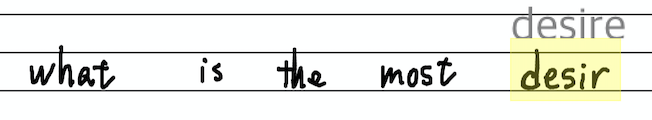
\includegraphics[scale=0.6]{images/word_region.png}
    \caption{region of interest detection works well when cutting out a word which is being written}
    \label{fig:cutting-word-region}
\end{figure}

On the other hand, when cutting out a handwritten illustration,
only a part of the illustration may be cut out if the lines constituting
the illustration are not spatially close to each other (Fig \ref{fig:failure}).

\begin{figure}
    \centering
    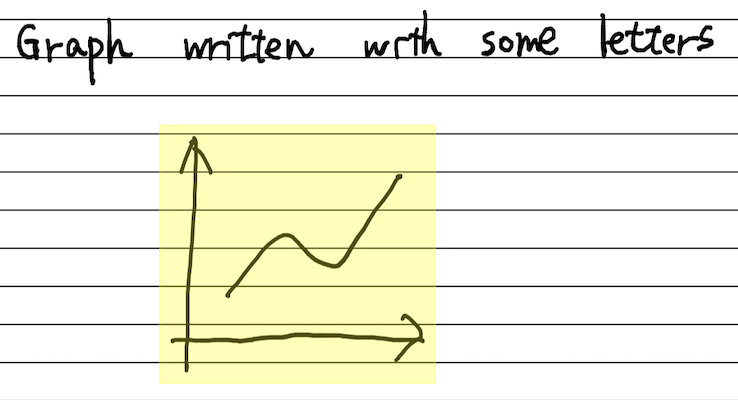
\includegraphics[scale=0.4]{images/illustration.png}
    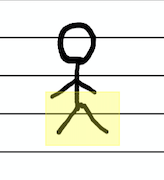
\includegraphics[scale=0.9]{images/failure.png}
    \caption{Left: example of the case ROI detection worked well on illustration. Right: example of failure case of ROI detection}
    \label{fig:failure}
\end{figure}

\subsection{Evaluation of Text recognition}
In the previous section, two patterns of text recognition were tried: recognition using
CTC and recognition using VNRecognizeText API. Since this report worked on recognition of
handwritten text and made use of the result for auto-complete, following metrics were
designed to measure the goodness of auto-completion.

\begin{itemize}
    \item Omitted Characters Count (OCC) - The gap between how many characters did the writer actually write before
    he found the word he wanted to write within top 10 of the auto-completion candidates
    and the number of characters in the word.
    If it is not found after writing to the end, the score is 0. Higher value of this metric indicates better result.
    \item Cumulative Time for Inference (CTI) - Cumulative time spent on auto-completion until the word that the writer actually
    wants to write is included in the top 10 auto-completion candidates. If it is not found after writing to the end,
    the score cumulative time spent on the recognition at each step. Note that each time writer releases the pen tip from the tablet, recognition
    process runs. Lower value of this metric indicates better result.
\end{itemize}

100 words were selected from the word list in /usr/share/dict/words of Debian GNU/Linux for evaluation.
Table \ref{tab:metrics} shows the performance of both methods on auto-completion. While OCC measure of
VNRecognizeText API show better result than CTC, cumulative time elapsed for inference is almost doubled
compared to that of CTC's.

\begin{table}[htbp]
    \centering
    \begin{tabular}{|l||c|c|} \hline
    method & OCC (mean) & CTI (mean) \\ \hline \hline
    CTC & 1.0102 & 1.1060 \\ \hline
    VNRecognizeText (.accurate) & 3.3405 & 1.9751 \\ \hline
    \end{tabular}
    \caption{Perfromance of CTC and VNRecognizeText API on auto-completion.}
    \label{tab:metrics}
\end{table}

\begin{figure}
    \centering
    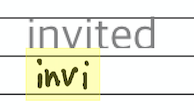
\includegraphics[]{images/auto-completion.png}
    \caption{Example of auto-completion showing the top 1 candidate}
    \label{fig:auto-complete}
\end{figure}

Figure \ref{fig:auto-complete} show an example of how auto-completion works.

\subsection{Discussion}

The VNRecognizeText API is superior to CTC in character recognition accuracy,
but in terms of speed it takes about three times longer to infer.
Since auto-completion is an application that requires real-time performance,
a small lag does not provide a good user experience. Therefore,
poor performance in speed can be a problem.

On the other hand, the CTC model shows inference speed that does not the user
feel uncomfortable in actual use, but the inference result is unstable,
and a slight difference in notation greatly affects the inference result.
Figure \ref{fig:unstable} shows an example of unstable inference.

\begin{figure}
    \centering
    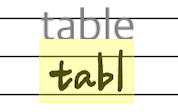
\includegraphics{images/table.png}
    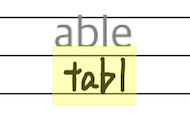
\includegraphics{images/able.png}
    \caption{Example of unstable inference}
    \label{fig:unstable}
\end{figure}

This is probably because training of the CTC model seems to be over-fitty
and strongly depends on the dataset used for training.
Therefore, future tasks include reducing the reliance on datasets and
using larger datasets or using data augmentation techniques to improve generalization performance.
